\documentclass{article}
\usepackage{graphicx}
\usepackage{amsmath}
\usepackage[parfill]{parskip}
\usepackage{hyperref}
\graphicspath{ {./figures/} }

\usepackage{biblatex}
\addbibresource{references.bib}

\title{COMP.SEC.220 Security Protocol\footnote{github --- \url{https://github.com/ancuongnguyen07/SecurityProtocol}}}
\author{Cuong Nguyen --- Coursework II}
\date{15/12/2022}

\begin{document}
    
\maketitle

\section{Experiment Results}
%
In this section, I evaluate the performance of the core algorithms of AinQ. I followed
exactly measurements and tried to re-generate the results in the given paper\cite{ainQ}.
In this experiment, I implemented the protocol on my personal laptop, a standard
machine which is commercially available. Both edge drones and a team leader
are operated on the same device.
Its specifications are shown in \autoref{tab:lap_spec}.

\begin{table}
    \centering
    \begin{tabular}{|l|l|}
        \hline
        Chipset & Apple Silicon M1 \\ \hline
        RAM & 16GB \\ \hline
        OS & MacOS Monterey 12.6.1 \\ \hline
    \end{tabular}
    \caption{My laptop specifications}\label{tab:lap_spec}
\end{table}

Respect to evaluate the performance of edge drones, \textbf{GenSecretValue} and
\textbf{KeyRetrieval} functions are focused. On the other hand, in terms of the performance
of team leader, \textbf{GenSecretValue, GenGroupKey} and \textbf{Re --- Key} functions
are focused.

\subsection{Edge Drone}
%
It is stated in the paper that the performance of the core functions on the resource-
constrained devices depends on the number of EC point multiplications\cite{ainQ}.
However, in the case of the standard powerful device, the difference is not obvious.
My laptop executed a single EC Multiplication in approximately 0.014 seconds, the
\textbf{GenSecretValue} in approximately 0.016 seconds, and the \textbf{KeyRetrival}
in approximately 0.015 seconds.

\begin{table}
    \centering
    \begin{tabular}{|c|c|c|}
        \hline
         & EM & Time (s) \\ \hline
        EC Multiplication & 0 & 0.014 \\ \hline
        GenSecretValue & 1 & 0.016 \\ \hline
        KeyRetrieval & 1 & 0.015 \\ \hline
    \end{tabular}
    \caption{Edge Drone Performance}\label{tab:edge_drone}
\end{table}

\subsection{Team Leader}
%
The performance of team leader is evaluated based on the execution time of two
core functions, \textbf{GenGroupKey} and \textbf{Re --- Key}. Hence, I measured
the execution time of the \textbf{GenGroupKey} function for a variying number
of existing edge drones, ranging from 1 to 2,000. In the case of only 1 edge
drone existed, \textbf{GenGroupKey} took approximately 0.044 seconds to execute
, while the number of edge drones was 2,000, it took 59.5 seconds to complete.
Due to the re-use of the same \emph{V} parameter for all edge drones, the execution
time increased in an efficient manner when I raised the number of edge drones.
In more detail, multiplying 0.044 seconds by 2,000 drones lead to approximately 88
seconds. As a result, I conclude that the \textbf{GenGroupKey} function obtained
about 40\% more efficient than the expected performance.

Respect to the \textbf{Re --- Key} algorithm, executed when an edge drone joins
the group, leaves the group or the current group key expires, I performed two
experiments to evaluate its performance. The first experiment focused on the key expiration.
For a variying
number of existing edge drones, ranging from 1 to 2,000, I measured the execution
time of the \textbf{Re --- Key} function. In the case of existing only 1 drone in
the group, it took 0.029 seconds to execute, while the number of edge drones was
2,000, the execution time was 0.094 seconds. \autoref{fig:team_leader} illustrates
the overall execution time of both the \textbf{GenGroupKey} and \textbf{Re --- Key}
functions for a variying number of edge drones, ranging from 1 to 2,000.

\begin{figure}[!ht]
    \centering
    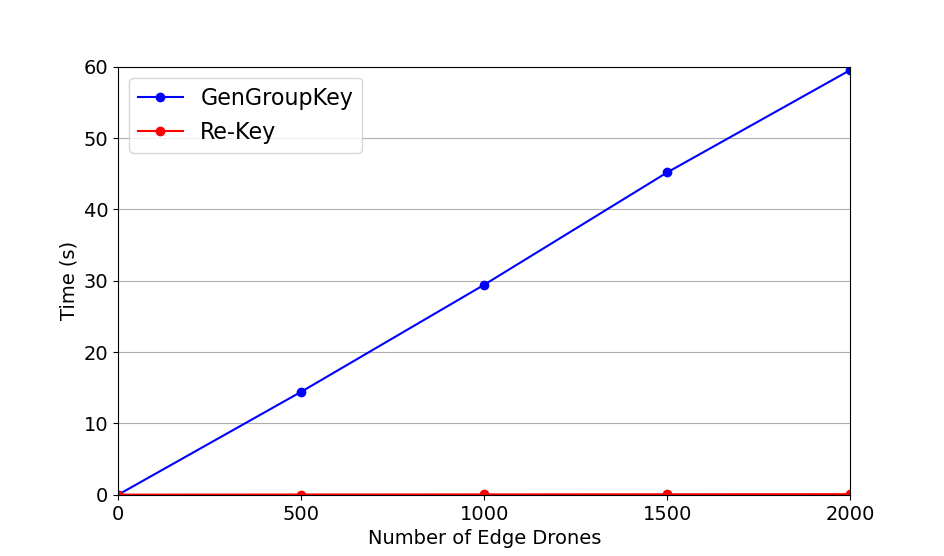
\includegraphics[height=\textheight,width=\textwidth,keepaspectratio]
    {leader_performance.png}
    \caption{Performance of the Team Leader}\label{fig:team_leader}
\end{figure}

For a second experiment, I measured the excution time of the \textbf{Re --- Key}
function when a variying number of new drones join a group including a variying
number of existing edge drones. When a new drone joins a group of only one member,
the \textbf{Re --- Key} took approximately 0.028 seconds to execute, while 1,000 new
drones join a group containing 1,000 existing drones, it took approximately 30.716
seconds. \autoref{tab:re_key} shows the results of these settings.

\begin{table}[!ht]
    \centering
    \begin{tabular}{|c|c|c|}
    \hline
        \textbf{Existing Group Members} & \textbf{New Group Members} & \textbf{Time (s)} \\ \hline
        1 & 1 & 0.028 \\
        1 & 100 & 2.919 \\
        1 & 500 & 14.463 \\
        1 & 1000 & 29.571 \\ \hline
        100 & 1 & 0.035 \\
        100 & 100 & 3.025 \\
        100 & 500 & 14.731 \\
        100 & 1000 & 29.913 \\ \hline
        500 & 1 & 0.047 \\ 
        500 & 100 & 2.990 \\
        500 & 500 & 15.143 \\
        500 & 1000 & 29.939 \\ \hline
        1000 & 1 & 0.064 \\
        1000 & 100 & 3.029 \\
        1000 & 500 & 15.252 \\
        1000 & 1000 & 30.716 \\ \hline
    \end{tabular}
    \caption{Group Re-key Function}\label{tab:re_key}
\end{table}

\section{Limitation and Future Work}
%
As you can see from the above experiment results, the execution time of core
functions in my implementation are much longer than those of authors' implementation.
The difference partly depends on the programming language and the cryptographic
library I utilized. Hence, I would try implement the protocol in Rust which has
better performance than Python, the programming language I utilized in this work.

\printbibliography{}

\end{document}